\section{Experiments and Results}

We simulate a two-dimensional SIR model with diffusion on a square domain \(\Omega = [0,L]\times [0,L]\) using a \(50\times 50\) grid.
The diffusion coefficients are set to \(\mu_S = 0.001\) and \(\mu_I = 0.001\), while the infection rate \(\beta=3.0\) is modified to be spatially and temporally dependent, as described in the previous section.

The initial conditions are chosen at random, with random positions for the infected individuals, and the simulation runs for \(T=15\).
At time \(t=8\), we introduce an event that increases the infection rate in the top half of the domain within a specific radius.

\begin{figure}[H]
  \centering
  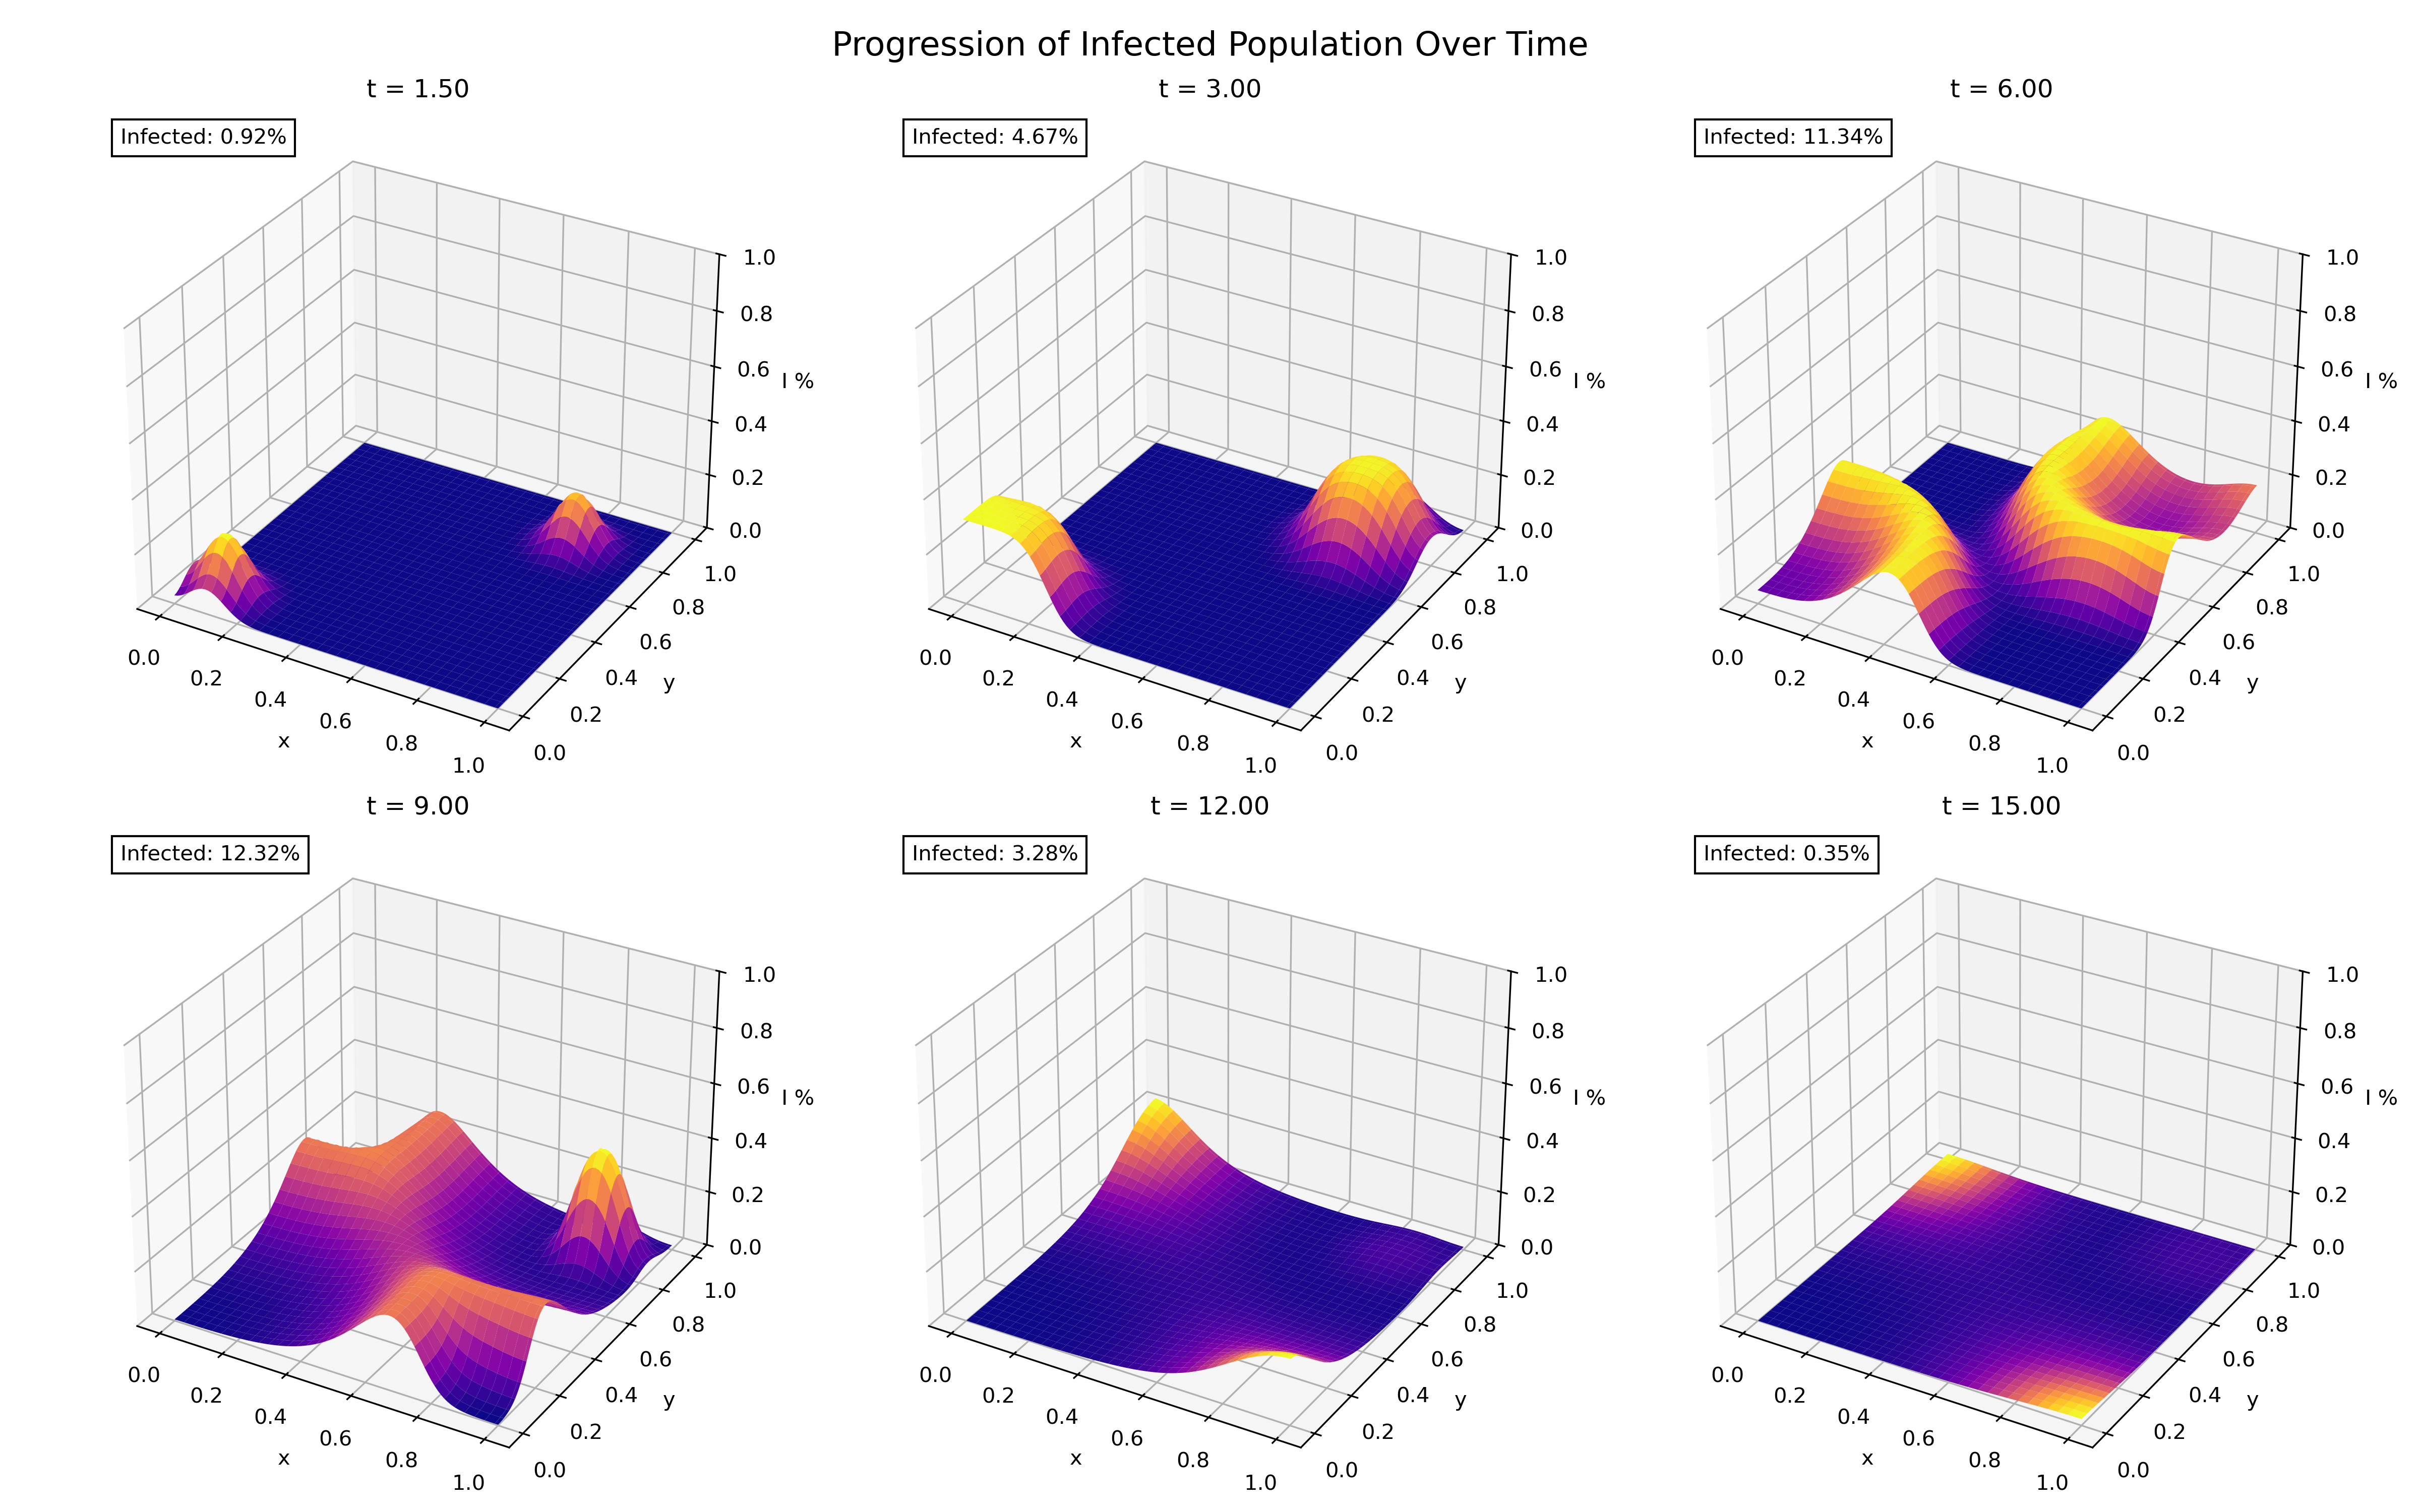
\includegraphics[width=1.0\textwidth]{figures/infected_progression.png}
  \caption{Progression of infected population over time.}
  \label{fig:infected_progression}
\end{figure}

We can see that the infected population increases rapidly from the initial conditions, and the event at \(t=8\) causes a significant local increase in the infected population.
The event is not strong enough to cause a global increase in the infected population, as most of the population has already recovered and the infection rate is still decreasing.
The event does, however, cause a local increase in the infected population, as can be seen in the figure.